\documentclass[12pt,border=6pt]{standalone}
\usepackage{fontspec}
\setmainfont{BeVietnamPro}[Path=D:/IOT_Tools/downloads/fonts/,Extension=.ttf,UprightFont=*-Regular,BoldFont=*-Bold]
\usepackage{amsmath}
\usepackage{unicode-math}\setmathfont{Cambria Math}
\usepackage{xcolor}
\usepackage{tikz}
\usetikzlibrary{positioning,arrows.meta,shapes.geometric,shapes.misc,calc,fit,backgrounds,decorations.pathreplacing,shadows,3d,perspective}
\usepackage{tikz-3dplot}
\usepackage{pgfplots}\pgfplotsset{compat=1.18}
\usepgfplotslibrary{groupplots,fillbetween}
\definecolor{cDo}{HTML}{BB2025}\definecolor{cDoD}{HTML}{8E1418}\definecolor{cDoT}{HTML}{FCEBEC}
\definecolor{cXanh}{HTML}{326CE5}\definecolor{cXanhT}{HTML}{EAF0FC}
\definecolor{cLuc}{HTML}{15803D}\definecolor{cLucT}{HTML}{E6F4EA}
\definecolor{cVang}{HTML}{B45309}\definecolor{cVangT}{HTML}{FDF2E1}
\definecolor{cNavy}{HTML}{1E293B}\definecolor{cMuc}{HTML}{1F2937}\definecolor{cXam}{HTML}{4B5563}
\definecolor{cXamT}{HTML}{F3F4F6}\definecolor{cVien}{HTML}{DDE1E6}\definecolor{cTim}{HTML}{6D28D9}\definecolor{cTimT}{HTML}{F1EBFD}
\pgfplotsset{slide/.style={tick label style={font=\small}, label style={font=\small}, scaled ticks=false,
  /pgf/number format/fixed, /pgf/number format/use comma, /pgf/number format/1000 sep={\,},
  legend style={font=\small,draw=none,fill=none}, axis line style={cXam}, major tick style={cXam},
  grid style={cVien}}}
\pgfkeys{/pgf/number format/assume math mode=true}
\begin{document}
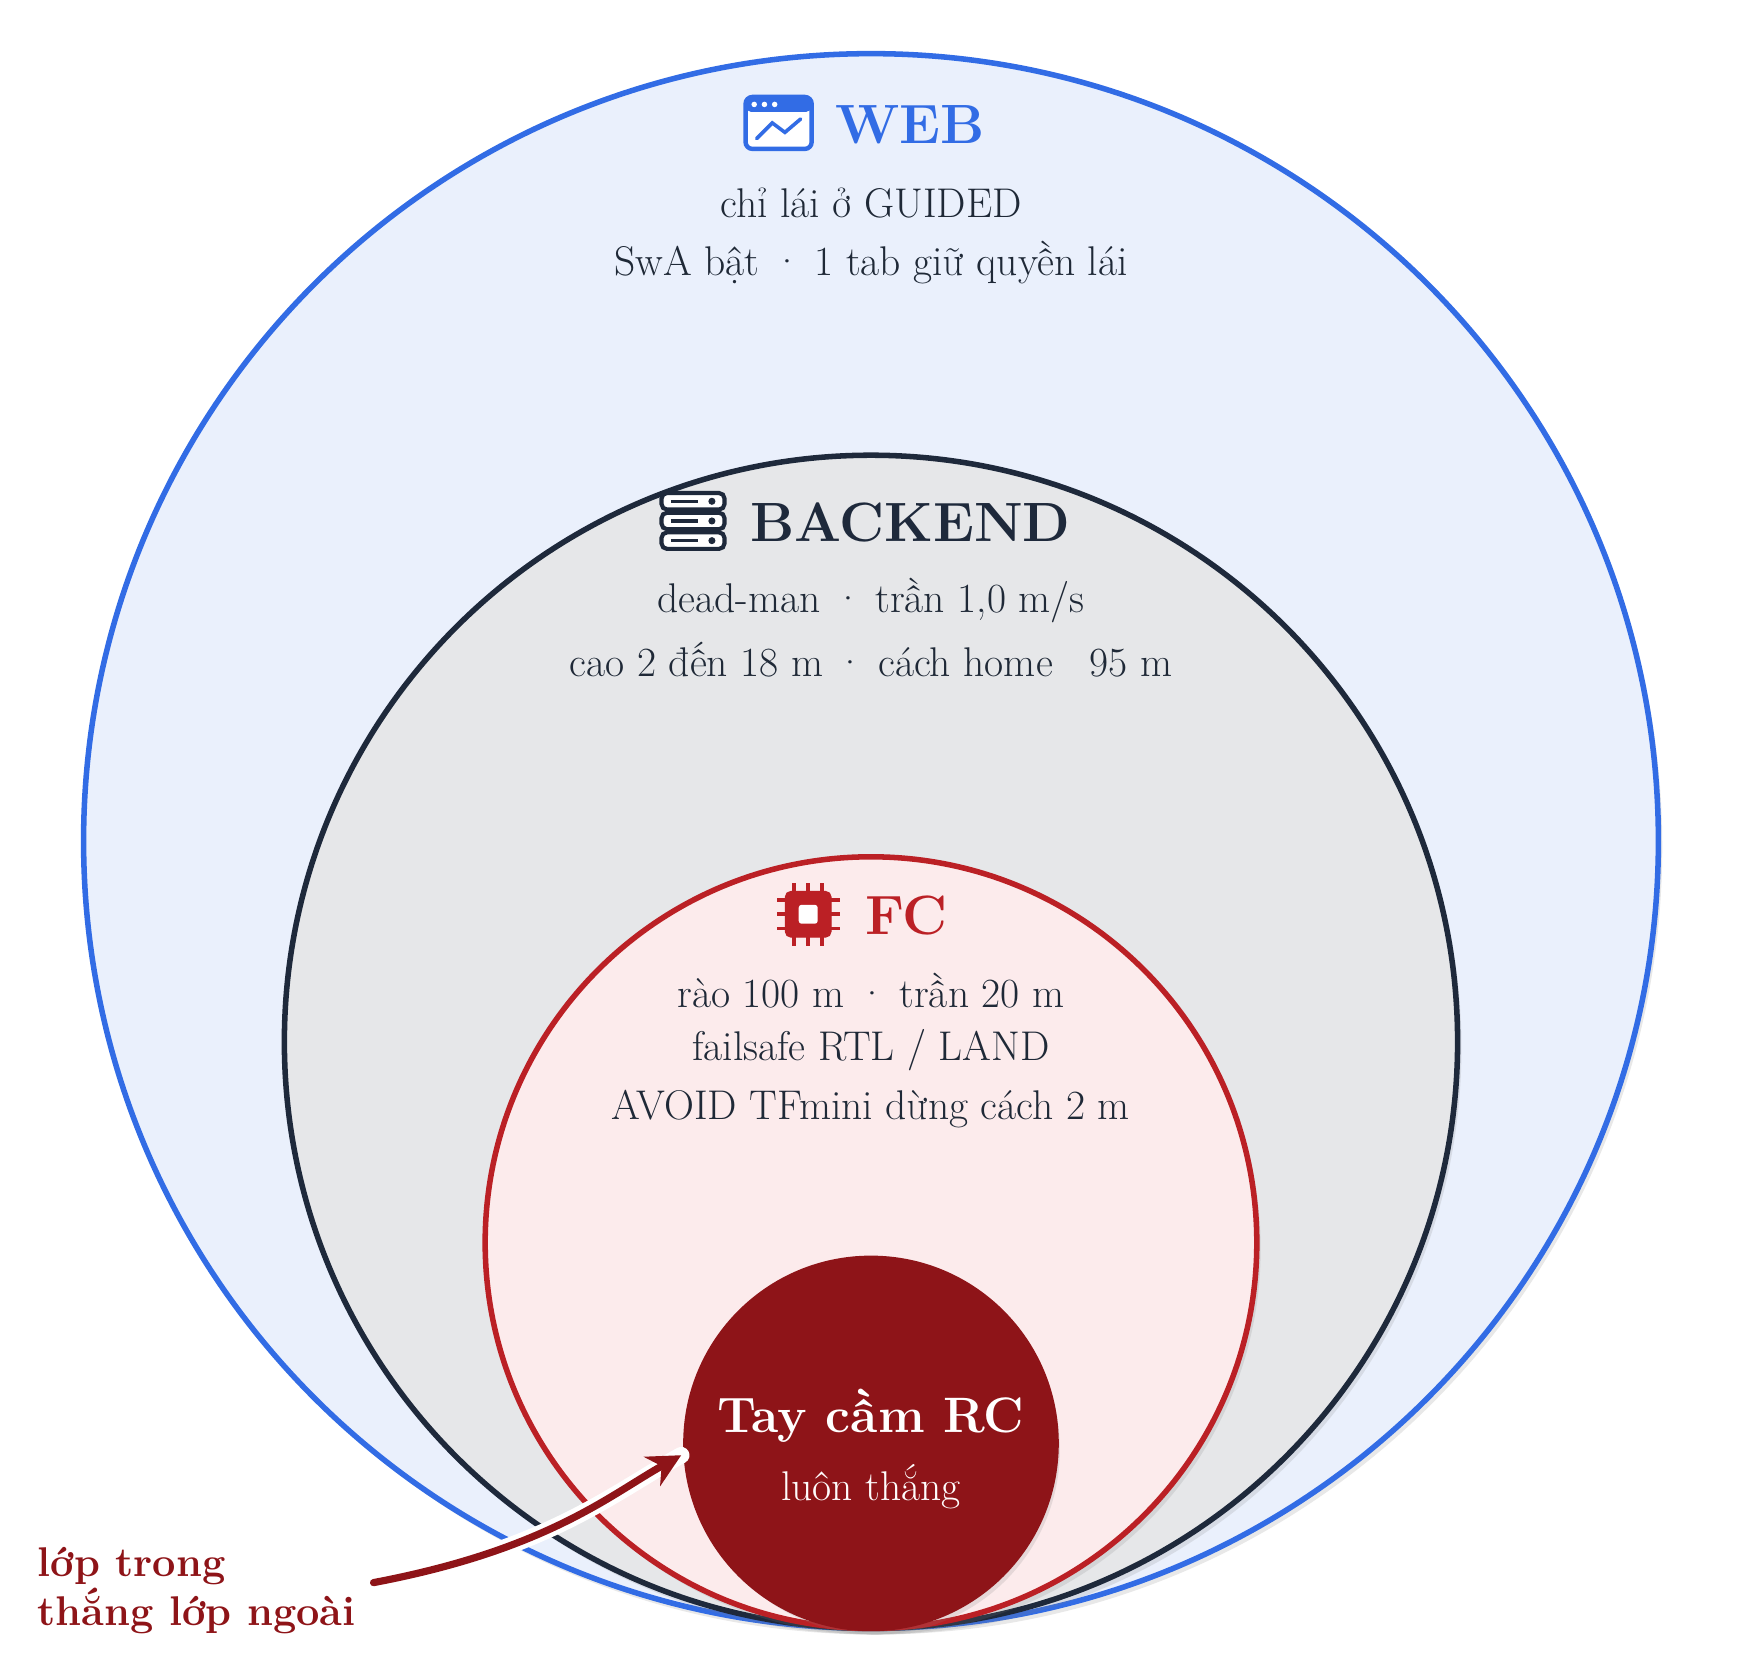
\begin{tikzpicture}[
  font=\fontsize{15}{18}\selectfont,
  shad/.style={drop shadow={opacity=0.18, shadow xshift=1.4pt, shadow yshift=-2.2pt}},
  ttl/.style={font=\bfseries\fontsize{20}{24}\selectfont},
  ln/.style={text=cMuc},
  ibrowser/.pic={
    \filldraw[fill=white, draw=#1, line width=1.6pt, rounded corners=2.5pt] (-0.42,-0.33) rectangle (0.42,0.33);
    \fill[#1, rounded corners=2pt] (-0.42,0.14) rectangle (0.42,0.33);
    \foreach \i in {0,1,2} \fill[white] (-0.31+\i*0.13,0.235) circle (0.035);
    \draw[#1, line width=1.3pt, line cap=round] (-0.28,-0.2) -- (-0.08,0.0) -- (0.08,-0.12) -- (0.28,0.05);
  },
  iserver/.pic={
    \foreach \j in {0,1,2}{
      \filldraw[fill=white, draw=#1, line width=1.5pt, rounded corners=2pt] (-0.4,-0.36+\j*0.25) rectangle (0.4,-0.15+\j*0.25);
      \fill[#1] (0.24,-0.255+\j*0.25) circle (0.045);
      \draw[#1, line width=1.2pt] (-0.28,-0.255+\j*0.25) -- (0.06,-0.255+\j*0.25);
    }
  },
  ichip/.pic={
    \foreach \k in {-0.18,0,0.18}{
      \draw[#1, line width=1.4pt] (\k,0.27) -- (\k,0.4); \draw[#1, line width=1.4pt] (\k,-0.27) -- (\k,-0.4);
      \draw[#1, line width=1.4pt] (0.27,\k) -- (0.4,\k); \draw[#1, line width=1.4pt] (-0.27,\k) -- (-0.4,\k);
    }
    \filldraw[fill=#1, draw=#1, rounded corners=2pt] (-0.29,-0.29) rectangle (0.29,0.29);
    \fill[white, rounded corners=1pt] (-0.12,-0.12) rectangle (0.12,0.12);
  },
]
\frenchspacing
% canvas 21,42 x 20,53 cm = the 8,6 x 8,25 in box of part_c (S21) minus the 6 pt border (scale 1 on the slide)
\def\W{21.42}\def\H{20.53}
\def\xc{10.71}\def\yb{0.2}
% nested circles, all touching the same bottom point
\filldraw[shad, fill=cXanhT, draw=cXanh, line width=2pt] (\xc,\yb+10.0) circle (10.0);
\filldraw[shad, fill=cNavy!11, draw=cNavy, line width=2pt] (\xc,\yb+7.45) circle (7.45);
\filldraw[shad, fill=cDoT, draw=cDo, line width=2pt] (\xc,\yb+4.9) circle (4.9);
\filldraw[shad, fill=cDoD, draw=cDoD, line width=2pt] (\xc,\yb+2.35) circle (2.35);
% web band
\node[ttl, text=cXanh] (tw) at (\xc+0.5,\yb+19.1) {WEB};
\pic at ($(tw.west)+(-0.6,0.02)$) {ibrowser=cXanh};
\node[ln] at (\xc,\yb+18.1) {chỉ lái ở GUIDED};
\node[ln] at (\xc,\yb+17.35) {SwA bật · 1 tab giữ quyền lái};
% backend band
\node[ttl, text=cNavy] (tb) at (\xc+0.5,\yb+14.05) {BACKEND};
\pic at ($(tb.west)+(-0.6,0.02)$) {iserver=cNavy};
\node[ln] at (\xc,\yb+13.05) {dead-man · trần 1,0 m/s};
\node[ln] at (\xc,\yb+12.3) {cao 2 đến 18 m · cách home ≤ 95 m};
% FC band
\node[ttl, text=cDo] (tf) at (\xc+0.45,\yb+9.05) {FC};
\pic at ($(tf.west)+(-0.6,0.02)$) {ichip=cDo};
\node[ln] at (\xc,\yb+8.1) {rào 100 m · trần 20 m};
\node[ln] at (\xc,\yb+7.35) {failsafe RTL / LAND};
\node[ln] at (\xc,\yb+6.6) {AVOID TFmini dừng cách 2 m};
% core
\node[text=white, align=center, font=\bfseries\fontsize{18}{21}\selectfont] at (\xc,\yb+2.7) {Tay cầm RC};
\node[text=white!85!cDoT, font=\fontsize{15}{18}\selectfont] at (\xc,\yb+1.8) {luôn thắng};
% inward arrow + label (bottom-left corner, outside the outer ring)
\node[anchor=south west, align=left, text=cDoD, font=\bfseries\fontsize{15}{18}\selectfont, inner sep=2pt] (lw) at (0.05,0.05) {lớp trong\\thắng lớp ngoài};
\draw[white, line width=6pt, line cap=round] ($(lw.east)+(0.15,0.1)$) .. controls (6.6,1.2) and (7.4,1.9) .. (8.3,2.4);
\draw[cDoD, line width=2.6pt, line cap=round, -{Stealth[length=12pt,width=12pt]}] ($(lw.east)+(0.15,0.1)$) .. controls (6.6,1.2) and (7.4,1.9) .. (8.3,2.4);
\pgfresetboundingbox
\useasboundingbox (0,0) rectangle (\W,\H);
\end{tikzpicture}

\end{document}
